\documentclass{standalone}

\usepackage{tikz}

\usetikzlibrary{positioning, chains, shapes.geometric, fit, shapes, arrows.meta, calc}

\begin{document}

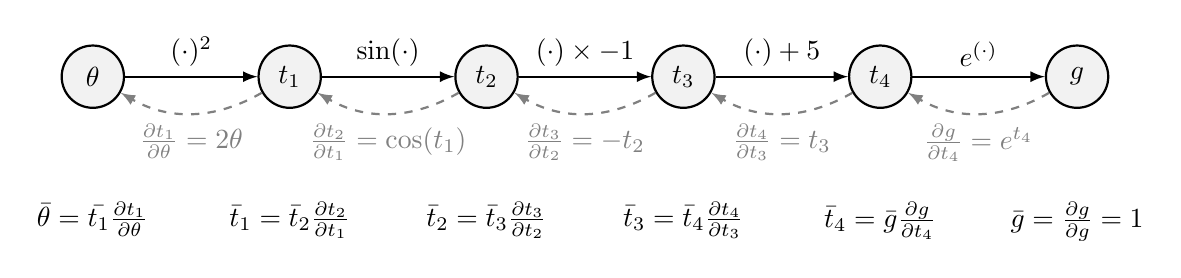
\begin{tikzpicture}[
    >=LaTeX, % Use default LaTeX arrows
    % Styles 
    node/.style={ % Input or output node
        circle,
        minimum width=2.25em,
        draw,
        fill=gray!10,
        thick
    },
    arrow/.style={
        -latex,
        thick
    },
    backprop/.style={ % Backpropagation arrows
        arrow,
        dashed,
        gray
    }
]
    % Computational graph nodes
    \node[node] (x) at (0,0) {$\theta$};
    \node[node] (x^2) at (2.5,0) {$t_1$};
    \node[node] (sin^2) at (5,0) {$t_2$};
    \node[node] (-sin^2) at (7.5,0) {$t_3$};
    \node[node] (+5) at (10,0) {$t_4$};
    \node[node] (exp) at (12.5,0) {$g$};
    
    % Computational graph edges
    \draw[arrow] (x) -- (x^2) node[midway, above] {$(\cdot)^2$};
    \draw[arrow] (x^2) -- (sin^2) node[midway, above] {$\sin(\cdot)$};
    \draw[arrow] (sin^2) -- (-sin^2) node[midway, above] {$(\cdot) \times -1$};
    \draw[arrow] (-sin^2) -- (+5) node[midway, above] {$(\cdot) + 5$};
    \draw[arrow] (+5) -- (exp) node[midway, above] {$e^{(\cdot)}$};

    % Adjoint calculations
    \node[below=3em of x] (dx) {$\bar{\theta} = \bar{t_1} \frac{\partial t_1}{\partial \theta}$};
    \node[below=3em of x^2] (dt1) {$\bar{t}_1 = \bar{t}_2 \frac{\partial t_2}{\partial t_1}$};
    \node[below=3em of sin^2] (dt2) {$\bar{t}_2 = \bar{t}_3 \frac{\partial t_3}{\partial t_2}$};
    \node[below=3em of -sin^2] (dt3) {$\bar{t}_3 = \bar{t}_4 \frac{\partial t_4}{\partial t_3}$};
    \node[below=3em of +5] (dt4) {$\bar{t}_4 = \bar{g} \frac{\partial g}{\partial t_4}$};
    \node[below=3em of exp] (dy) {$\bar{g} = \frac{\partial g}{\partial g} = 1$};

    % Backpropagation arrows with partial derivatives
    \draw[backprop, bend left=30] (x^2) to node[midway, below] {$\frac{\partial t_1}{\partial \theta} = 2\theta$} (x);
    \draw[backprop, bend left=30] (sin^2) to node[midway, below] {$\frac{\partial t_2}{\partial t_1} = \cos(t_1)$} (x^2);
    \draw[backprop, bend left=30] (-sin^2) to node[midway, below] {$\frac{\partial t_3}{\partial t_2} = -t_2$} (sin^2);
    \draw[backprop, bend left=30] (+5) to node[midway, below] {$\frac{\partial t_4}{\partial t_3} = t_3$} (-sin^2);
    \draw[backprop, bend left=30] (exp) to node[midway, below] {$\frac{\partial g}{\partial t_4} = e^{t_4}$} (+5);
\end{tikzpicture}

\end{document}